\documentclass{article}
\usepackage[legalpaper, margin=0.5in]{geometry} % Changing margin sizes
\usepackage{graphicx, lmodern, tikz, wrapfig} % Required for images

\setcounter{secnumdepth}{0} % Removes section numbering


\title{Kepler's Laws of Planetary Motion}

\date{\vspace{-12ex}}
\begin{document}

\maketitle


\begin{figure}[!hb]
\centering
\label{curve}
    \includegraphics[scale=0.20]{Kepler.png}
\begin{minipage}[b]{5cm}
\begin{trivlist}  
\item Johannes Kepler was a German astronomer and mathematician who was born in 1571 and died in 1630. He discovered three laws of celestial mechanics and he published them between the years of 1609 and 1619. Kepler later became an assistant to the astronomer Tycho Brahe and Kepler improved upon Gallileo's telescope design.
\end{trivlist}
\end{minipage}
\end{figure}




\section*{\centering{Kepler's 1st law}}

Kepler's 1st law states that the planets move in elliptical orbits with the Sun at one of the foci. 
Mathematically stated in polar coordinates, the equation of an ellipse with the sun at one focus is given by: 

$$r(\theta) = \frac{l}{1+ecos(\theta)}$$

Where: 
$r(\theta)$ is the distance from the planet to the Sun at a specific angle $\theta$.
$\ell$ is the semi-latus rectum of the ellipse.
e is the eccentricity of the ellipse, which measures how "stretched out" the ellipse is. \newline

Starting with the total energy of an orbit, which is the kinetic energy and potential energy we have $$E = \frac{1}{2}mv^2 - \frac{GMm}{r}$$

Converting this to polar coordinates, 

$$v^2 = (\dot{r}^2 + r^2{\dot{\theta}}^2) \rightarrow E = \frac{1}{2}m(\dot{r}^2 + r^2{\dot{\theta}}^2) - \frac{GMm}{r} $$

Using the equation for angular momentum L, we can rearrange to have an equation for $\dot{\theta}$

$$L = mvr = m r^2 \dot{\theta} \rightarrow \dot{\theta} = \frac{L}{mr^2}$$

Taking the integral of $\dot{\theta}$ we get 

$$\theta = \int \dot{\theta} dt = \int \frac{L}{mr^2} dt \rightarrow r_{inverse} = r_i = \frac{1}{r} \rightarrow \dot{r} = \frac{-1}{r_i^2} \frac{dr_i}{dt} \rightarrow \theta = -\int \frac{L}{m \dot{r}} dr_i$$

Now we will rearrange the equation for the total energy of the orbit and solve for $\dot{r}$

$$E = \frac{1}{2}m(\dot{r}^2 + r^2{\dot{\theta}}^2) - \frac{GMm}{r} 
 \rightarrow \dot{r^2} = \frac{2E}{m} + \frac{GMm}{r} - \frac{L^2r_i^2}{m^2}$$

Now, we must define the semi-latus rectum and the eccentricity of the ellipse to further simplify the derivation.

$$\ell = \frac{L^2}{GMm^2}$$ $$e = \sqrt{1 + \frac{2E\ell}{GMm}}$$

\begin{center}
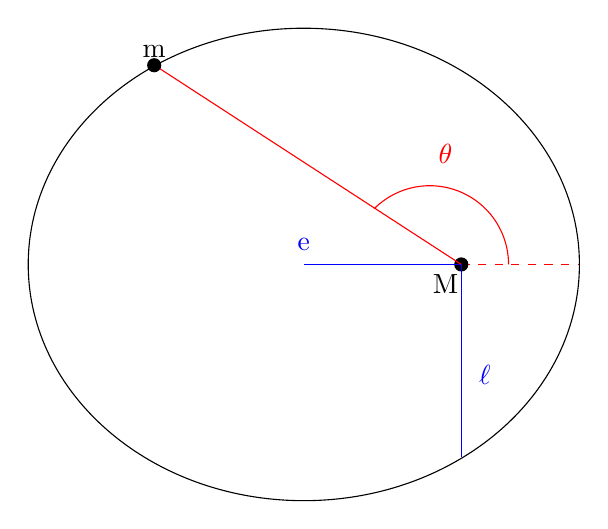
\begin{tikzpicture}
    \draw (0,0) ellipse (3.5cm and 3 cm);

    \draw [red] [dashed] (2,0) -- (3.5,0); %dashed line on right
    \node [scale=1] at (1.8, -0.25) {M}; mass, M at the right focus.
    \fill[black] (2,0) circle(.09);

    \draw[blue] (0,0) -- (2,0); %line from right focus to center
    \node[blue] [scale=1] at (0,0.25) {e}; % describing the ecentricity
    
    \draw [red] (2,0) -- (-1.85,2.5); % line from right focus to mass, m
    \node[scale=1] at (-1.9,2.7) {m};
    \fill[black] (-1.9,2.53) circle(.09);

    \draw [blue] (2,0) -- (2,-2.45);
    \node [blue] [scale=1] at (2.3, -1.4) {$\ell$};

    \draw[red] (2.6, 0) arc[start angle=0, end angle=135, radius=1]; %theta arc
    \node[red] [scale=1] at (1.8, 1.4) {$\theta$};

\end{tikzpicture}
\end{center}



Rewriting the expression from before with the new values of $\ell$ and e, we have

$$\dot{r^2} = \frac{2E}{m} + \frac{GMm}{r} - \frac{L^2r_i^2}{m^2} = \frac{L}{m}\sqrt{\frac{e^2}{\ell^2}-(r_i - \frac{1}{\ell})^2}$$

Using the previous formula for $\theta$ we can further simplify and then integrate.

$$\theta = -\int \frac{L}{m \dot{r}} dr_i = -\int \frac{dr_i}{\sqrt{(\frac{e}{\ell})^2 - (r_i-\frac{1}{\ell})^2}} = cos^{-1}(\frac{r_i - \frac{1}{\ell}}{\frac{e}{\ell}})$$

Finally, after taking the integral, we can find a function, r of theta which describes an elliptical orbit

$$ \theta = cos^{-1}(\frac{r_i - \frac{1}{\ell}}{\frac{e}{\ell}}) \rightarrow cos(\theta) = (\frac{1}{r} - \frac{1}{\ell}) \frac{\ell}{e} \rightarrow r = \frac{\ell}{1 + e cos(\theta)}$$

\section*{\centering{Kepler's 2nd law}}

Kepler's 2nd law states that a line segment joining a planet and the Sun sweeps out equal areas during equal time intervals. In other words, the rate at which a planet moves along its orbit it sweeps out area remains constant. This law stated mathematically is $\frac{dA}{dt} = Constant$ \newline

\begin{center}
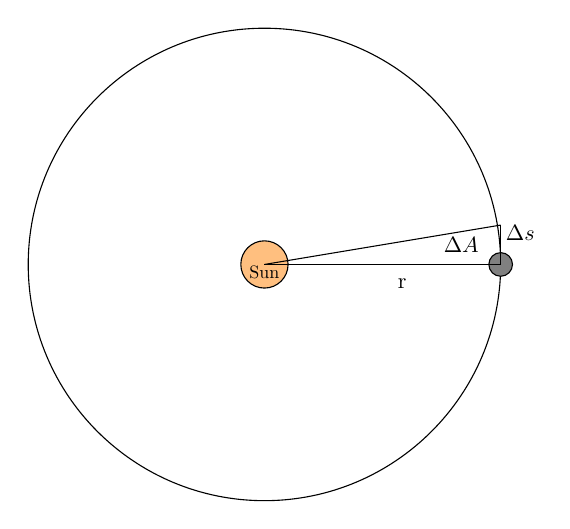
\begin{tikzpicture}
    \draw (0,0) circle (3);
    \draw[fill=orange, fill opacity=0.5] (0,0) circle (0.3);
    
    \node[scale=0.65] at (0,-0.1) {Sun};
    
    \draw[scale=0.5, fill=gray, fill opacity=1] (6,0) circle (0.3);
    
    \draw (3,0) -- (3,0.5);
    \node[scale=0.8] at (3.25,0.40) {$\Delta s$};
    
    \draw (0,0) -- (3,0);
    \node[scale=0.8] at (1.75,-0.25) {r};

    \draw (0,0) -- (3, 0.5);
    \node [scale=0.8] at (2.5, 0.25) {$\Delta A$};
\end{tikzpicture}
\end{center}


\newline

The area of a triangle is given by the formula $A = \frac{1}{2} base * height$ thus, $\Delta A \approx \frac{1}{2} r * \Delta s \rightarrow \frac{dA}{dt} = \frac{1}{2} r \frac{ds}{dt} \rightarrow s = r \theta \rightarrow \frac{dA}{dt} = \frac{1}{2} r^2 \frac{d\theta}{dt}$ \newline

$\frac{dA}{dt}$ represents the rate at which the planet sweeps out area, and $\frac{d\theta}{dt}$ is the angular speed of the planet. \newline

Angular momentum is defined as $L = m v r$ and arc length is defined as $s = r \theta$. The tangential velocity is directly related to the rate of change of the angle $\theta$ as it moves around the sun with $v = \frac{ds}{dt} = r \frac{d\theta}{dt}$. Substituting in for the formula for angular momentum, we have $L = m \frac{ds}{dt} = r \frac{d\theta}{dt} r = m \frac{ds}{dt} = r^2 \frac{d\theta}{dt}$ \newline

Since angular momentum is constant, $r^2 \frac{d\theta}{dt}$ must also be constant. Since we proved earlier that $\frac{dA}{dt} = \frac{1}{2} r^2 \frac{d\theta}{dt}$ $\frac{dA}{dt}$ must also be constant, proving Kepler's 2nd law.


\section*{\centering{Kepler's 3rd law}}

Kepler's 3rd law states that the square of a planet's orbital period is proportional to the cube of the length of the semi-major axis of its orbit, written mathematically, $T^2 \propto r^3$ \newline

This proportion can be deduced starting with Newton's universal law of gravitation and using algebraic manipulation \newline

$F = \frac{GM_sM_p}{r^2} = M_pa \rightarrow M_pa_c$ Since we are discussing orbital mechanics, we must use centripetal acceleration. \newline

Centripetal acceleration can be derived by $a_c = \frac{2\pi v}{\frac{2 \pi r}{v}} = \frac{v^2}{r}$ \newline

\begin{center}
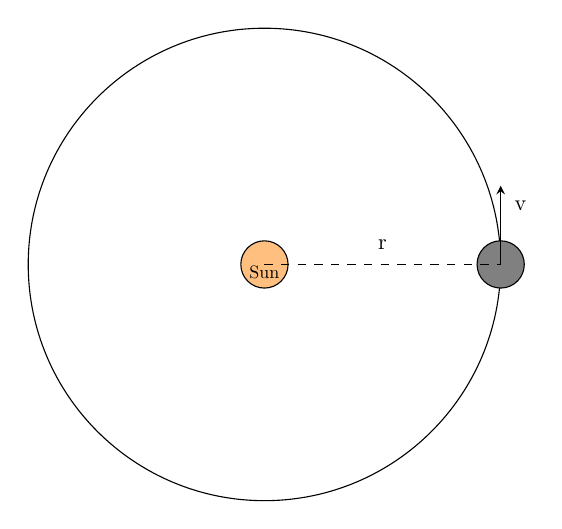
\begin{tikzpicture}
    \draw (0,0) circle (3);
    \draw[fill=orange, fill opacity=0.5] (0,0) circle (0.3);
    \node[scale=0.65] at (0,-0.1) {Sun};
    \draw[fill=gray, fill opacity=1] (3,0) circle (0.3);
    \draw [-stealth](3,0) -- (3,1);
    \node[scale=0.8] at (3.25,0.75) {v};
    \draw [dashed] (0,0) -- (3,0);
    \node[scale=0.8] at (1.5,0.25) {r};
\end{tikzpicture}
\end{center}

Tangential velocity can be defined as distance over time. The distance a planet travels in 1 orbit is $2\pi$ at a distance of the semi-major axis, r, and the time period will be denoted as T. Thus $v = \frac{2\pi r}{T}$ \newline

$\sum F = M_p a_c = \frac{M_p v^2}{r} = \frac{M_p ({\frac{2 \pi r}{T}})^2}{r} = \frac{M_p 4 \pi r^2}{r T^2}$ \newline

Equating the derived force equation with the semi-major axis, r, and the period, T, with the universal law of gravitation, will reveal the proportionality. \newline

$\sum F = \frac{M_p 4 \pi r}{T^2} = \frac{GM_sM_p}{r}\rightarrow T^2 = \frac{4 \pi r^3}{G M_s} \rightarrow T^2 \propto r^3$






\end{document}
